\section{Methods}

In this section, we derive the discretized equations for the initial and boundary value problem and describe the OCI iteration.
We have chosen to implement robust second-order discretization methods: simple corner balance  \cite{adams_subcell_1997} in space and multiple balance \cite{variansyah_robust_2021} in time.
By coupling these higher accuracy schemes with an efficient iterative method, we hope to optimize the ratio of compute work to communication work to better suit the numerical method for GPUs.
To confirm that multiple balance time discretization remains unconditionally stable with simple corner balance, we conduct Fourier analysis for a non-scattering model problem.
Then, we derive the Fourier system for a single time step of simple corner balance + multiple balance discretization using both OCI and SI operator splitting to study the convergence rate.
Finally, we present systems for multi-group transport.

\subsection{Derivation of space and time discretization for one-cell inversion}
\label{sec:methods-derv}
We begin with the time-dependent, isotropic scattering slab geometry, S$_N$ transport equations with an isotropic source.
\begin{multline}
    \label{eq:sn_nte}
    \frac{1}{v} \frac{\partial \psi_{m}(x,t)}{\partial t} + \mu_m \frac{\partial \psi_{m}(x,t)}{\partial x} + \Sigma(x) \psi_{m}(x,t) 
     = \frac{1}{2} \left( \Sigma_{s}(x) \sum\limits_{n=1}^N w_n \psi_{n}(x,t) + Q(x,t) \right) \;, \\
    \qquad \qquad m=1, \ldots, N \;, \qquad t > 0 \;, \qquad x \in [0,X]
\end{multline}
where $\psi$ is the angular flux, $t$ is time, $x$ is location, $v$ is speed, $\Sigma$ is the macroscopic total cross-section, $\Sigma_s$ is the macroscopic scattering cross-section, $w_m$ is angular quadrature weight, $\mu_m$ is the angular quadrature ordinate, $m$ is the quadrature index, $N$ is the quadrature order, and $Q$ is the isotropic material source.
The initial and boundary conditions are prescribed angular flux distributions:
\begin{equation*}
    \psi_{m}(x,0) = \psi_{init,m}(x), \qquad m=1 \ldots N \;,
\end{equation*}
\begin{equation*}
    \psi_{m}(0,t) = \psi_{inc,m}^+(t), \qquad \mu_m >0 \;,
\end{equation*}
\begin{equation*}
    \psi_{m}(X,t) = \psi_{inc,m}^-(t), \qquad \mu_m <0 \;.
\end{equation*}

We discretize these equations in time using multiple balance~\cite{variansyah_robust_2021}, which solves two coupled sets of equations. 
First is a backward Euler step (transport equation integrated over a time step):
\begin{subequations}
\begin{multline}
\frac{1}{v} \left( \frac{\psi_{m,k+1/2}(x) - \psi_{m,k-1/2}(x)}{\Delta t} \right) + \mu_m \frac{\partial \psi_{m,k}(x)}{\partial x} + \Sigma(x) \psi_{m,k}(x) \\
= \frac{1}{2} \left(  \Sigma_{s}(x) \sum\limits_{n=1}^N w_n \psi_{n,k}(x) + Q_{k}(x) \right) \;,
\end{multline}
and the second is a balance like auxiliary equation from the multiple balance principle:
\begin{multline}
\frac{1}{v} \frac{\psi_{m,k+1/2}(x) - \psi_{m,k}(x)}{\Delta t/2} + \mu_m \frac{\partial \psi_{m,k+1/2}(x)}{\partial x} + \Sigma(x) \psi_{m,k+1/2}(x) \\
= \frac{1}{2} \left( \Sigma_{s}(x) \sum\limits_{n=1}^N w_n \psi_{n,k+1/2}(x) + Q_{ k+1/2}(x) \right) \;,
\end{multline}
\end{subequations}
where $\Delta t$ is the time step size, $k$ indicates time-average quantities, and $k\pm1/2$ indicates time-edge quantities.
Then, we discretize in space using simple corner balance, which involves a spatial integration over the right and left halves of a spatial cell:
\begin{subequations}
\label{eq:scb-mb}
\begin{multline}
\label{eq:scb-mb-a}
\frac{\Delta x_j}{2} \frac{1}{v} \left( \frac{\psi_{m,k+1/2,j,L} - \psi_{m,k-1/2,j,L}}{\Delta t} \right)
 + \mu_m \left[ \frac{\left( \psi_{m,k,j,L} + \psi_{m,k,j,R} \right)}{2}  - \psi_{m,k,j-1/2} \right] \\
+ \frac{\Delta x_j}{2} \Sigma_{j} \psi_{m,k,j,L} 
= \frac{\Delta x_j}{2} \frac{1}{2} \left( \Sigma_{s,j} \sum\limits_{n=1}^N w_n \psi_{n,k,j,L} + Q_{k,j,L} \right) \;,
\end{multline}  
\begin{multline}
\label{eq:scb-mb-b}
\frac{\Delta x_j}{2} \frac{1}{v} \left( \frac{\psi_{m,k+1/2,j,R} - \psi_{m,k-1/2,j,R}}{\Delta t} \right) +
\mu_m \left[ \psi_{m,k,j+1/2} - \frac{\left( \psi_{m,k,j,L} + \psi_{m,k,j,R} \right)}{2}   \right] \\
+ \frac{\Delta x_j}{2} \Sigma_{j} \psi_{m,k,j,R} = \frac{\Delta x_j}{2} \frac{1}{2} \left( \Sigma_{s,j} \sum\limits_{n=1}^N w_n \psi_{n,k,j,R} + Q_{k,j,R} \right) \;,
\end{multline}  
\begin{multline}
\label{eq:scb-mb-c}
\frac{\Delta x_j}{2} \frac{1}{v} \left( \frac{\psi_{m,k+1/2,j,L} - \psi_{m,k,j,L}}{\Delta t/2} \right) \\
+ \mu_m \left[ \frac{\left( \psi_{m,k+1/2,j,L} + \psi_{m,k+1/2,j,R} \right)}{2}  - \psi_{m,k+1/2,j-1/2} \right]
+ \frac{\Delta x_j}{2} \Sigma_{j} \psi_{m,k+1/2,j,L} \\
= \frac{\Delta x_j}{2} \frac{1}{2} \left( \Sigma_{s,j} \sum\limits_{n=1}^N w_n \psi_{n,k+1/2,j,L} + Q_{k+1/2,j,L} \right) \;,
\end{multline}    
\begin{multline}
\label{eq:scb-mb-d}
\frac{\Delta x_j}{2} \frac{1}{v} \left( \frac{\psi_{m,k+1/2,j,R} - \psi_{m,k,j,R}}{\Delta t/2} \right) + \\
\mu_m \left[ \psi_{m,k+1/2,j+1/2} - \frac{\left( \psi_{m,k+1/2,j,L} + \psi_{m,k+1/2,j,R} \right)}{2}   \right]
+ \frac{\Delta x_j}{2} \Sigma_{j} \psi_{m,k+1/2,j,R} \\
= \frac{\Delta x_j}{2} \frac{1}{2} \left( \Sigma_{s,j} \sum\limits_{n=1}^N w_n \psi_{n,k+1/2,j,R} + Q_{k+1/2,j,R} \right) \;,
\end{multline} 
\end{subequations}
where $\Delta x$ is the cell width, $j$ is the spatial cell index, $L/R$ is the left or right half cell, respectively.
These equations contain the first of the two simple spatial closures---the angular flux at the cell midpoint is a simple average of the two half-cell average quantities:
\begin{subequations}
\begin{equation}
  \psi_{m,k}(x_j) =  \frac{\left( \psi_{m,k,j,L} + \psi_{m,k,j,R} \right)}{2} \;,
\end{equation}
\begin{equation}
  \psi_{m,k+1/2}(x_j) =  \frac{\left( \psi_{m,k+1/2,j,L} + \psi_{m,k+1/2,j,R} \right)}{2} \;.
\end{equation}
\end{subequations}
The second closure is an \textit{upstream} prescription for the cell-edge angular flux:
\begin{subequations}
\begin{equation}
  \psi_{m,k,j+1/2} =
  \begin{cases}
  \psi_{m,k,j,R}, & \mu_m > 0, \\
  \psi_{m,k,j+1,L}, & \mu_m < 0 \;,
  \end{cases}
\end{equation}
\begin{equation}
  \psi_{m,k+1/2,j+1/2} =
  \begin{cases}
  \psi_{m,k+1/2,j,R}, & \mu_m > 0, \\
  \psi_{m,k+1/2,j+1,L}, & \mu_m < 0 \;.
  \end{cases}
\end{equation}
\end{subequations}
Figure \ref{fig:stencil} shows the stencil location for angular flux and source terms. 
\begin{figure}[!htb]
    \centering
    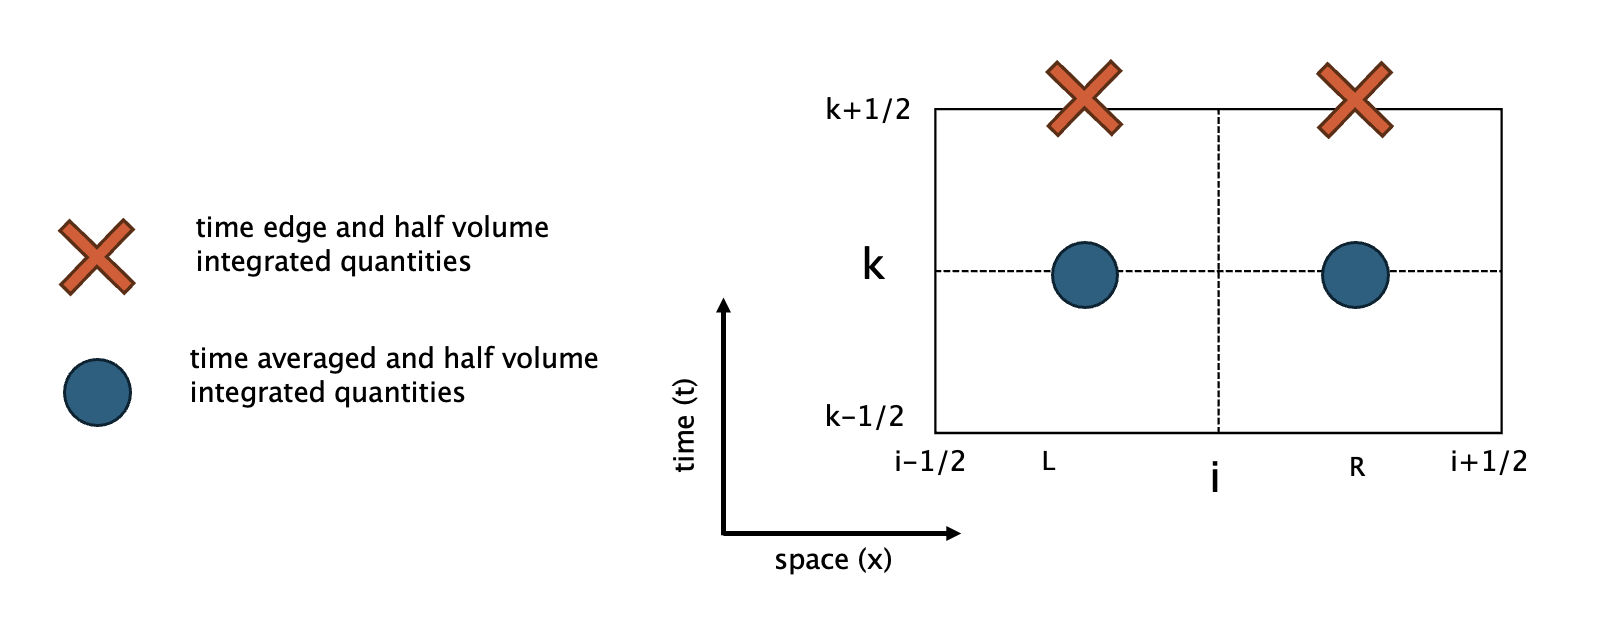
\includegraphics[width=\textwidth]{manuscript2/man2_figs/stencil.png}
    \caption{Discretization stencil for simple corner balance, multiple balance time discretization}
    \label{fig:stencil}
\end{figure}

Solving Eq.~\eqref{eq:scb-mb} iteratively requires operator splitting.
Unknown values (from the current iteration, noted by $l+1$) are moved to the left-hand side to form a large system of linear equations.
In SI, the scalar flux in the scattering source is evaluated at the previous iteration $(l)$, decoupling angles and coupling space.
OCI allows the fluxes incident to the cell---defined by upstream closures---to lag, thus decoupling cells from one another within an iteration.

In OCI, the scattering source is subtracted to the left-hand side and  prior iteration values are employed for all information incident on cell $j$ (moved to the right-hand side).
This means that all $4N$ angular fluxes ($N$ angles at $L$ and $R$, $k$ and $k+1/2$) are computed simultaneously in cell $j$.
This yields a linear system for each cell $j$:
\begin{equation}
    \label{eq:oci}
    \left( \bm{L}_{c,j} - \bm{S}_j \right) \Psi_j^{(l+1)} = -\textbf{L}_{b,j} \Psi_j^{(l)} + \textbf{Q} \;, 
\end{equation}
where $l$ is the iteration index.
The right-hand side can be combined into a known vector
\begin{equation}
     \left( \bm{L}_{c,j} - \bm{S}_j \right) \Psi_j^{(l+1)}  = \bm{b}_j \; ,
\end{equation}
where $\bm{L}_{c,j}$ and $\bm{S}_j$ are both of size $4N\times4N$ and likewise $\bm{b}_j$ is a vector of length $4N$.
\newcommand{\lcmj}[1]{\begin{bmatrix} \bm{L}_{c,j,#1} \end{bmatrix} }
\newcommand{\zeros}{\begin{bmatrix} 0 \end{bmatrix} }
The within-cell operator is
\begin{subequations}
\begin{equation}
    \label{eq:Aja}
    \bm{L}_{c,j} = \begin{bmatrix}
        \lcmj{1} &  &  &  &  \\
          & \ddots  &  &  & \\
          &  & \lcmj{m} &  & \\
          &  &  & \ddots &  \\
          &  &  &  & \lcmj{N}
    \end{bmatrix} \;,
\end{equation}
with zeros elsewhere, where
\begin{equation} \bm{L}_{c,j,m} =
    \label{eq:Aj}
    \begin{bmatrix}
    \frac{|\mu_m| + \Delta x_j \Sigma_{j} }{2}  & \frac{\mu_m}{2} & \frac{\Delta x_j}{2 v \Delta t} & 0 \\
    - \frac{\mu_m}{2} & \frac{|\mu_m| +  \Delta x_j \Sigma_{j,g} }{2} & 0 & \frac{\Delta x_j}{2 v \Delta t} \\
    -\frac{\Delta x_j}{v \Delta t}  & 0 & \frac{\Delta x_j}{v \Delta t} + \frac{|\mu_m| + \Delta x_j \Sigma_{j,g} }{2}  & \frac{\mu_m}{2}  \\
    0 &  -\frac{\Delta x_j}{v \Delta t}  &  - \frac{\mu_m}{2} & \frac{\Delta x_j}{v \Delta t}+ \frac{|\mu_m| + \Delta x_j \Sigma_{j,g}}{2}  \\
    \end{bmatrix} \; .
\end{equation}
\end{subequations}
The right-hand side is
\begin{subequations}
\begin{equation}
    \bm{b}_j =  \left[
    \bm{b}_{j,1} \; \bm{b}_{j,2} \; \cdots \; \bm{b}_{j,N} \right]^{T} \;.
\end{equation}
As the linear system in each cell contains contributions from all angles (both positive and negative) $b_{j,m}$ is given by
\begin{equation} 
    \bm{b}_{j,m} = 
    \begin{cases}
        \bm{b}_{j,m}^+ & \mu_m>0 \\
        \bm{b}_{j,m}^- & \mu_m<0 \\
    \end{cases} \;,
\end{equation}
where
\begin{equation}
     \bm{b}_{j,m}^+ = \begin{bmatrix}
     \frac{\Delta x_j}{4} Q_{k,j,L} + \frac{\Delta x_j}{2 v \Delta t} \psi_{m,k-1/2,j,L} + \mu_m \psi^{(l)}_{m,k,j-1,R} \\
     \frac{\Delta x_j}{4}Q_{k,j,R} + \frac{\Delta x_j}{2 v \Delta t} \psi_{m,k-1/2,j,R} \\
     \frac{\Delta x_j}{4}Q_{k+1/2,j,L} + \mu_m \psi^{(l)}_{m,k+1/2,j-1,R} \\
     \frac{\Delta x_j}{4} Q_{k+1/2,j,R} 
    \end{bmatrix} \;,
\end{equation}
and
\begin{equation}
    \bm{b}_{j,m}^- = \begin{bmatrix}
    \frac{\Delta x_j}{4}  Q_{k,j,L} + \frac{\Delta x_j}{2 v \Delta t} \psi_{m,k-1/2,j,L}  \\
    \frac{\Delta x_j}{4}  Q_{k,j,R} + \frac{\Delta x_j}{2 v \Delta t} \psi_{m,k-1/2,j,R} - \mu_m \psi^{(l)}_{m,k,j+1,L}  \\
    \frac{\Delta x_j}{4}  Q_{k+1/2,j,L}  \\
    \frac{\Delta x_j}{4}  Q_{k+1/2,j,R} - \mu_m \psi^{(l)}_{m,k+1/2,j+1,L}
    \end{bmatrix} \;.
\end{equation}
\end{subequations}
The elements of the ${S_j}$ matrix are defined by
\begin{equation}
    \label{eq:scatter}
   [\mathbf{S}_j]_{k.l} = \begin{cases}
			\frac{\Delta x_j \Sigma_{s,j}}{4}w_{|(l-k)|/3)}, & \text{if $\mod{\frac{(l-k)}{3} =0}$}\\
            0, & \text{otherwise}
		 \end{cases} \; ,
%  \frac{\Delta x_j \Sigma_{s,j}}{4} w_n \;
\end{equation}
where $w$ are the angular quadrature weights.
%To adapt this scheme to anisotropic scattering regimes alterations to $S_j$ would be required.
Finally,
\begin{subequations}
\begin{equation}
\Psi^{(l+1)}_j =  \begin{bmatrix}
    \bm{\psi}_{j,1}^{(l+1)}, \;
    \bm{\psi}_{j,2}^{(l+1)}, \;
    \cdots \;
    \bm{\psi}_{j,N}^{(l+1)}
    \end{bmatrix} ^{T} \; ,
\end{equation}
where
\begin{equation} 
\bm{\psi}_{j,n}^{(l+1)} = \begin{bmatrix}
    \psi_{n,k,j,L}^{(l+1)}, \;
    \psi_{n,k,j,R}^{(l+1)}, \;
    \psi_{n,k+1/2,j,L}^{(l+1)}, \;
    \psi_{n,k+1/2,j,R}^{(l+1)}
    \end{bmatrix}^{T} \;.
\end{equation}
\end{subequations}
One-cell inversion iterations continue until
\begin{equation}
    ||\Psi^{(l+1)}-\Psi^{(l)}||_{2} < \epsilon(1-\rho_e) \; ,
\end{equation}
where $\epsilon$ is the convergence tolerance and
\begin{equation}
    \rho_e = \frac{||\Psi^{(l+1)}-\Psi^{(l)}||_{2}}{||\Psi^{(l)}-\Psi^{(l-1)}||_{2}}
\end{equation}
is an empirical estimation of the spectral radius computed at every iteration of a transport solve.
After convergence, the time-step counter increments and the time-step process can be repeated.

Generally, Jacobi and Gauss--Seidel iterations converge faster when a system is more diagonally dominant \cite{isaacson_numerical_1966, golub_matrix_1983}.
Equation~\eqref{eq:Aj} contains ($ \delta/2 = \Delta x\Sigma/2 $) on the diagonals.
So in the thin limit (when $\delta\rightarrow 0$) the system becomes overall less diagonally dominant and converges more slowly.
However Equation~\eqref{eq:Aj} also involves $\Delta x/(v\Delta t)$ terms in elements (3,3) and (4,4).
Thus, a smaller time step will cause the system to become more diagonally dominant.
We provide a similar description of simple corner balance and multiple balance time discretization for an unpreconditioned source iteration \cite{morgan2023oci}.


\subsection{Fourier analysis: time-stepping scheme}


To ensure that the combination of higher-order discretization schemes remains an unconditionally stable time-marching method, we perform Fourier analysis (also known as Von Neumann stability analysis)~\cite{leveque2007finite}.
A time marching scheme
\begin{equation}
    \Psi_{k+1/2} = \bm{K} \Psi_{k-1/2} \;,
\end{equation}
where $\bm{K}$ is the time iteration matrix, is unconditionally stable when the Von Neumann stability condition is met:
\begin{equation}
    \sup(|\lambda_{K}|) \leq 1 \;,
    \label{eq:unconstab}
\end{equation}
where $\lambda_K$ are the eigenvalues of $\bm{K}$ \cite{golub_matrix_1983, isaacson_numerical_1966}.
$\bm{K}$ can be derived for a given model problem.
We consider a model problem consisting of a homogeneous infinite medium with no scattering to derive the eigenfunction of the time-dependent multiple balance, simple corner balance discretization scheme.
Since this problem has no scattering, each angle can be solved independently of every other angle, and no operator splitting is required.
We first start by describing the absolute error of the angular flux at time step $(k+1/2)$:
\begin{equation}
    \mathbf{f}_{k+1/2} = \Psi_{\text{exact}} - \Psi_{k+1/2} \;.
\end{equation}
Then, we define a Fourier ansätz for the error propagated through a time step:
\begin{subequations}
\begin{align}
    f_{k+1/2,j,L} &= \lambda^{k+1}a_t e^{i\omega j} \; ,
    &
    f_{k+1/2,j,R} &= \lambda^{k+1}b_t e^{i\omega j} \; ,
\end{align}
\begin{align}
    f_{k,j,L} &= \lambda^{k}c_t e^{i\omega j} \; ,
    &
    f_{k,j,R} &= \lambda^{k}d_t e^{i\omega j} \; ,
\end{align}
\begin{align}
    f_{k-1/2,j,L} &= \lambda^{k}a_t e^{i\omega j} \; ,
    &
    f_{k-1/2,j,R} &= \lambda^{k}b_t e^{i\omega j} \; ,
\end{align}
\end{subequations}
where $k$ is the time step, $i=\sqrt{-1}$, $\lambda$ is the eigenvalue, $\omega$ is the wave number, $j$ is cell index and $a_t$, $b_t$, $c_t$, and $d_t$ are components of the eigenvector.
Substituting our ansätz into the error form of Eqs.~\eqref{eq:scb-mb} and assuming $\mu>0$, we simplify to form:
\begin{subequations}
\begin{equation}
    \label{eq:eig1}
    \frac{\Delta x}{2} \frac{1}{v \Delta t} (\lambda a_t- a_t) + \mu \left(\frac{c_t+d_t}{2} - d_t e ^{-i\omega} \right) + \frac{\Sigma\Delta x }{2}c_t = 0 \; ,
\end{equation}
\begin{equation}
\label{eq:eig2}
    \frac{\Delta x}{2} \frac{1}{v \Delta t} (\lambda b_t - b_t) + \mu \left( c_te^{i\omega} - \frac{c_t+d_t}{2} \right) + \frac{\Sigma\Delta x }{2}d_t = 0 \; ,
\end{equation}
\begin{equation}
\label{eq:eig3}
    \frac{\Delta x}{2} \frac{2}{v \Delta t} (\lambda a_t - c_t) + \lambda\mu \left( \frac{a_t+b_t}{2} - b_t e^{-i\omega} \right) + \frac{\Sigma\Delta x }{2}a_t \lambda = 0 \; ,
\end{equation}
\begin{equation}
\label{eq:eig4}
    \frac{\Delta x}{2} \frac{2}{v \Delta t} (\lambda b_t - d_t) + \lambda\mu \left( d_t e^{i\omega} + \frac{c_t+d_t}{2} \right) + \frac{\Sigma\Delta x}{2} b_t\lambda = 0 \;,
\end{equation}
\end{subequations}
combining Eq.~\eqref{eq:eig1} into \eqref{eq:eig2}:
\begin{equation}
    \label{eq:f_a-1}
    \begin{bmatrix}
        c_t\\d_t
    \end{bmatrix}
    = \bm{K_{+}}^{-1} \frac{\Delta x}{2}\frac{1}{v\Delta t}(1-\lambda)
    \begin{bmatrix}
        a_t\\b_t
    \end{bmatrix} \;,
\end{equation}
where
\begin{equation}
    {\bm{K_{+}}} = 
    \begin{bmatrix}
    \frac{\mu}{2}+\frac{\Sigma \Delta x}{2} & \mu (\frac{1}{2} - e^{-i\omega}) \\
    -\frac{\mu}{2} & \frac{\mu}{2}+\frac{\Sigma \Delta x}{2}
    \end{bmatrix} \;.
\end{equation}
Then, doing the same with Eq.~\eqref{eq:eig3} into \eqref{eq:eig4}:
\begin{equation}
    \label{eq:f_a-2}
    \lambda \left( \bm{K_{+}} + \frac{\Delta x}{v \Delta t} \bm{I} \right)  \begin{bmatrix}
        a_t \\ b_t
    \end{bmatrix} = \frac{\Delta x}{v\Delta t} \begin{bmatrix}
        c_t \\ d_t
\end{bmatrix} \; ,
\end{equation}
where $\bm{I}$ is the identity matrix. Combining Eq.~\eqref{eq:f_a-1} into \eqref{eq:f_a-2} gives
\begin{equation}
    \lambda
    \begin{bmatrix}
        a_t \\b_t
    \end{bmatrix}
    = \left[ \bm{K_{+}} + \frac{\Delta x}{v\Delta t} \bm{I} + \gamma\bm{K_{+}}^{-1} \right]^{-1} \gamma \bm{K_{+}}^{-1}
    \begin{bmatrix}
        a_t \\ b_t
    \end{bmatrix} \; ,
\end{equation}
where $\gamma = \frac{\Delta x}{v\Delta t}  \frac{\Delta x}{2v\Delta t}$.
This can then be more appropriately posed as an eigenfunction:
\begin{equation}
    \lambda_K
    \bm{a}
    = \bm{K} \bm{a}\;,
\end{equation}
where
\begin{equation}
    \bm{K} = \gamma \left( \bm{K_{+}}\bm{K_{+}} + \frac{\Delta x}{v \Delta t}\bm{K_{+}} + \gamma \bm{I}\right)^{-1}
\end{equation}
and the eigenvector is
\begin{equation}
    \bf{a} = \begin{bmatrix}
        a_t, & b_t
    \end{bmatrix} ^T \;.
\end{equation}
The analysis is similar for $\mu<0$ only with
\begin{equation}
    \bm{K_{-}} = \begin{bmatrix}
        -\frac{\mu}{2} + \frac{\Sigma\Delta x}{2} & \frac{\mu}{2} \\
        \mu \left ( e^{i\omega} - \frac{1}{2} \right) & -\frac{\mu}{2} + \frac{\Sigma\Delta x}{2} 
    \end{bmatrix} \;.
\end{equation}

This system can be numerically solved after making discrete selections of $\mu \in [-1, 1]$ and $\omega \in (0,2\pi]$ at a point in the perameter space ($\Delta x$, $\Delta t$, $v$, $\Sigma$) with \texttt{numpy.max(numpy.abs(numpy.linalg.eig(K))}~\cite{harris2020array}.

Figure \ref{fig:mb-scb} shows the absolute value of the maximum eigenvalues of $\bm{K}$ at various points in mean free time ($\tau=\Sigma v\Delta t$) and cellular optical thickness ($\delta=\Sigma\Delta x$) at 75 discrete points $\omega \in (0,2\pi]$ in S$_{16}$.
None of $|\lambda_{max}|$ are above one, which means the Von Neumann stability criterion in Eq. \eqref{eq:unconstab} is satisfied and the combination of the multiple balance time discretization and the simple corner balance scheme is unconditionally stable for this infinite homogeneous medium problem with no scattering.
%While experimenting with this method we did find that, under some conditions, it can produce negative fluxes; however, the negative flux oscillations are critically damped and dissipate with time.

\begin{figure}[htbp]
    \centering
    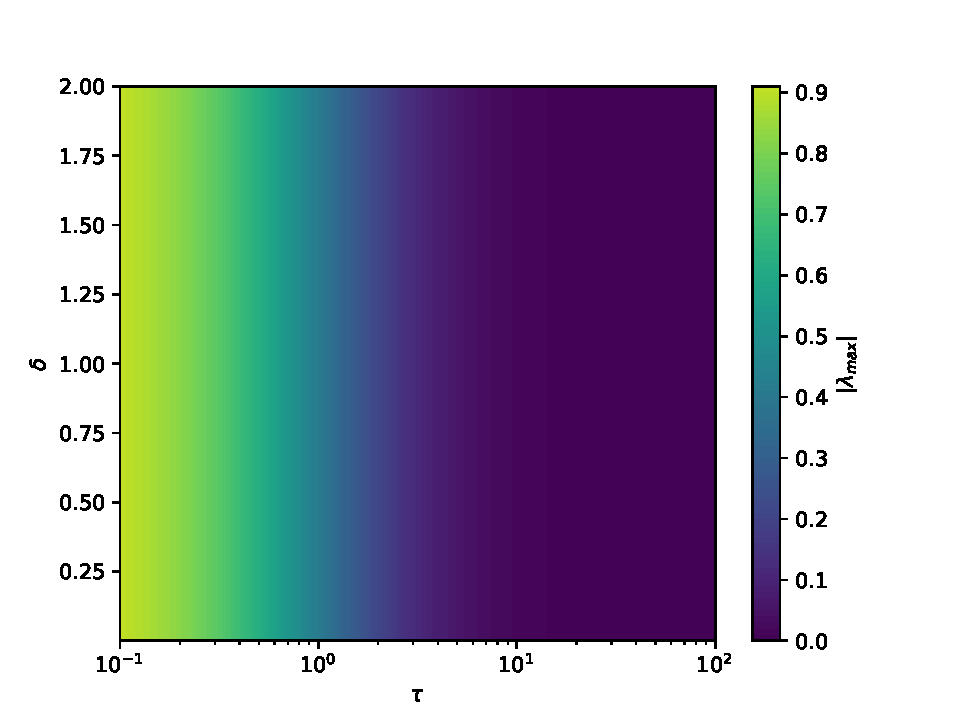
\includegraphics[width=0.75\linewidth]{manuscript2/man2_figs/mb_scb.pdf}
    \caption{$|\lambda_{\max}|$ from numerically solved multiple balance time discretization and simple corner balance Fourier system over choices in mean free time ($\tau$) and cellular optical thickness ($\delta$) in S$_{16}$.}
    \label{fig:mb-scb}
\end{figure}


\subsection{Fourier analysis: OCI iterative scheme}
\label{sec:methods-faoci}



\newcommand{\exi}{e^{i\lambda\Sigma x_j}}
\newcommand{\omlp}{\omega^{(l+1)}}
\newcommand{\oml}{\omega^{(l)}}
\newcommand{\dx}{\Delta x}
\newcommand{\dt}{\Delta t}
\newcommand{\scatsum}{\sum^{M}_{n=0}}


To study the impact of time dependence on the convergence of an OCI iteration, we conduct a Fourier analysis on the error equation of an infinite-homogeneous medium model problem in slab geometry in a single time step.
Similar to the analysis in the previous section, we can assert that for an iteration scheme
\begin{equation}
    \Psi^{(l+1)} = \bm{T} \Psi^{(l)} \;,
\end{equation}
where $(l)$ is the iteration counter, convergence rate is
\begin{equation}
   \rho = \sup(|\lambda_{\bm{T}}|)\;,
\end{equation}
 where $\lambda_{\bm{T}}$ contains the eigenvalues of $\bm{T}$ \cite{golub_matrix_1983, isaacson_numerical_1966}.
An iterative method will converge if and only if $\rho<1$. 
Furthermore, iterations converge faster for smaller $\rho$.

To derive the transport matrix $\bm{T}$ we can again use Fourier separation analysis on a model problem.
We first start by describing the absolute error of the angular flux at iteration step $(l)$
\begin{equation}
    \mathbf{f}^l = \Psi^{\text{converged}} - \Psi^l \;,
\end{equation}
and our Fourier anzats on a functional form of that error
\begin{subequations}
    \label{eq:anz}
    \begin{align}
        f^{(l)}_{m,k,j,L/R} &= \omega^{(l)}a_{m,L/R}e^{i\lambda\Sigma x_j} \; ,
        &
        f^{(l)}_{m,k+1/2,j,L/R} &= \omega^{(l)}b_{m,L/R}e^{i\lambda\Sigma x_j} \;.
    \end{align}
\end{subequations} 
The upstream closures at the left boundary of the cell are
\begin{subequations}
\begin{equation}
    f_{m,k,j-1/2} =
    \begin{cases}
        f_{m,k,j-1, R} \;, & \mu > 0 \\
        f_{m,k,j, L} \;, & \mu < 0 
    \end{cases} \;,
\end{equation}
and at the right are
\begin{equation}
    f_{m,k,j+1/2} =
    \begin{cases}
        f_{m,k,j, R} \;, & \mu > 0 \\
        f_{m,k,j+1, L} \;, & \mu < 0 
    \end{cases} \;.
\end{equation}
\end{subequations}

\iffalse
\begin{subequations}
    \begin{align}
        f^{(l)}_{m,k,j-1/2} &= f^{(l)}_{m,j-1,R} \; ,
        &
        f^{(l+1)}_{m,k,j+1/2} &= f^{(l+1)}_{m,k,j,R} \; ,
    \end{align}
    \begin{align}
        f^{(l)}_{m,k+1/2,j-1/2} &= f^{(l)}_{m,k+1/2,j-1,R} \; ,
        &
        f^{(l+1)}_{m,k+1/2,j+1/2} &= f^{(l+1)}_{m,k+1/2,j,R} \; ,
    \end{align}
\end{subequations}
where $i=\sqrt{-1}$. Note only the \textit{incident} flux is lagged.
Similarly, for negative directions ($\mu_m<0$):
\begin{subequations}
    \begin{align}
        f^{(l+1)}_{m,k,j-1/2} &= f^{(l+1)}_{m,j,L} \; ,
    &
        f^{(l)}_{m,k,j+1/2} &= f^{(l)}_{m,k,j+1,L} \; ,
    \end{align}
    \begin{align}
        f^{(l+1)}_{m,k+1/2,j-1/2} &= f^{(l+1)}_{m,k+1/2,j,L} \; ,
        &
        f^{(l)}_{m,k+1/2,j+1/2} &= f^{(l)}_{m,k+1/2,j+1,R} \; .
    \end{align}
\end{subequations}
\fi

Now, substitute the ansätz and upstream closures into the error form of Eq. \eqref{eq:scb-mb} and derive the eigensystem.
This is done by (1) collecting like terms, (2) dividing both sides by $\omega^{(l)} e^{i\Sigma x_j}$, (3) isolating terms with a remaining $\omega$ to the left-hand side, and finally (4) forming the eigensystem into the iteration matrix over all angular directions:
\begin{equation}
    \bm{T}_{OCI} = \left( 
    \bm{L}_c
    - \bm{S}
    \right)^{-1}
    \begin{bmatrix}
        \bm{L}_b^- & 0\\
        0 & \bm{L}_b^+
    \end{bmatrix} \;,
\end{equation}
which now forms a well-posed eigenvalue problem over all angles:
\begin{equation}
    \lambda\bm{a} = \bm{T} \bm{a} \; ,
\end{equation}
where the eigenvector $\mathbf{a}$ is defined by
\begin{equation}
    \mathbf{a} = \begin{bmatrix}
        a_{1} & a_{2} & \cdots & a_M
    \end{bmatrix} ^T \;,
\end{equation}
\begin{equation}
    a_m = \begin{bmatrix}
        a_{mR} & a_{mL} & b_{mR} & b_{mL} 
    \end{bmatrix} ^T \; ,
\end{equation}
$\bm{L}_c$ is the linear within-cell transport operator defined by Eqs.~\eqref{eq:Aja} and \eqref{eq:Aj}, 
\begin{equation}
    \bm{L}_b^+ = 
    \begin{bmatrix}
        0 & 0 & 0 & 0 \\
        -\mu_m e^{-i\lambda\sigma\dx} & 0 & 0 & 0 \\
        0 & 0 & 0 & 0 \\
        0 & 0 & -\mu_m e^{-i\lambda\sigma\dx} & 0
    \end{bmatrix} \; ,
\end{equation}
and
\begin{equation}
    \bm{L}_b^- = 
    \begin{bmatrix}
        0 & \mu_m e^{i\lambda\sigma\dx} & 0 & 0 \\
        0 & 0 & 0 & 0 \\
        0 & 0 & 0 & \mu_m e^{i\lambda\sigma\dx} \\
        0 & 0 & 0 & 0
    \end{bmatrix} \; .
\end{equation}
The scattering matrix is again akin to the previously described transport matrix in Eq.~\eqref{eq:scatter}.
Finally, to numerically evaluate the spectral radius we form the system for a given set of angles and weights from Gauss--Legendre quadrature and solve with \texttt{numpy.max(numpy.abs(numpy.linalg.eig(T)))} for $\omega \in [0,2\pi]$ at discrete points.
We vary the cellular optical thickness ($\delta =\Sigma \Delta x$), mean free time ($\tau = \Sigma v\Delta t$), and scattering ratio ($c=\Sigma_s/\Sigma$) to study convergence behavior in various physical regimes. 
The analogous eigensystem for source iteration is
\begin{equation}
    \bm{T}_{SI} = \left( 
    \bm{L}_c
    + \begin{bmatrix}
        \bm{L}_b^- & 0\\
        0 & \bm{L}_b^+
    \end{bmatrix}
    \right)^{-1}
    \bm{S} \; .
\end{equation} 
Section~\ref{sec:results-faoci} contains the results of this analysis.


\subsection{OCI multi-group transport}

We extend our single energy derivations presented in Section~\ref{sec:methods-derv} to be energy dependent. 
Elements of the $\mathbf{S_{g' \rightarrow g}}$ matrix are now defined by
%\begin{equation}
%    \bm{S}_{g\rightarrow g',n} = \frac{\Delta x_j \Sigma_{s,g'\rightarrow g,j}}{4} w_n \;,
%\end{equation}
\begin{equation}
    \label{eq:scatter}
   [\mathbf{S}_{g' \rightarrow g,j}]_{k.l} = \begin{cases}
			\frac{\Delta x_j \Sigma_{s,g'\rightarrow g,j}}{4}w_{|(l-k)|/3)}, & \text{if $\mod{\frac{(l-k)}{3} =0}$}\\
            0, & \text{otherwise}
		 \end{cases} \; ,
%  \frac{\Delta x_j \Sigma_{s,j}}{4} w_n \;
\end{equation}
where $g' \rightarrow g$ indicates transfer from group $g'$ to group $g$ and $w$ are the quadrature weights. 
The systems described in Section~\ref{sec:methods-derv} now include multi-group scattering:
\begin{equation}
    \bm{A}_j = 
    \begin{bmatrix}
        \bm{L}_{c,j,1} -\bm{S}_{1\rightarrow1,j} & -\bm{S}_{2\rightarrow1,j} & \cdots & \cdots& -\bm{S}_{G\rightarrow1,j}\\
        -\bm{S}_{1\rightarrow2,j} & \ddots & & & \vdots\\
         \vdots & & \bm{L}_{c,j,g}-\bm{S}_{g\rightarrow g,j} &  & \vdots\\
        \vdots & &  &  \ddots & \vdots \\
        -\bm{S}_{1\rightarrow G,j} & \cdots & \cdots & & \bm{L}_{c,j,G} -\bm{S}_{G\rightarrow G,j}
    \end{bmatrix} \; ,
\end{equation}
where
\begin{equation}
    \bm{b}_j = 
    \begin{bmatrix}
        b_{j,1}, & b_{j,2}, & \cdots, & b_{j,G}
    \end{bmatrix} ^T \; .
\end{equation}

\begin{figure}[htbp]
    \centering
    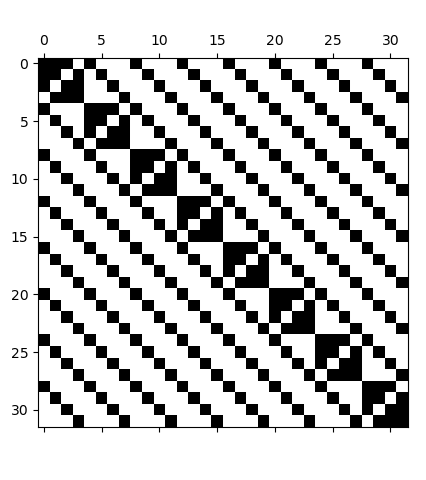
\includegraphics[width=.6\textwidth]{manuscript2/man2_figs/spyA.png}
    \caption{Sparsity pattern of a two group, four angle OCI $\bm{A}_j$ system generated for each cell.}
    \label{fig:spyA}
\end{figure}

Figure~\ref{fig:spyA} shows the structure of the within-cell system of equations arises from a two-group four-angle problem.
While $A_j$ does have significant sparsity,  with an occupancy ratio of
\begin{equation}
    O_c = \frac{G(N+2)}{4NG}
    \; ,
\end{equation}
in this work we use dense representations in each cell because the matrix memory size for 1D transport is not limiting.

\subsection{Implementation on GPUs}



Implementing the OCI and SI approaches on GPUs requires a numerical linear algebra solver library like LAPACK~\cite{laug}.
Many high-performance open-source linear algebra tools exist (e.g., Trillinos, PETSc, SUNDIALS, MAGMA), but we chose a vendor-supplied package depending on the hardware target of choice.
Our target hardware is an AMD MI250X so we use the AMD ROCm compute library to solve the system of equations.
Modern GPU vendor-supplied LAPACK libraries often include a \texttt{batched} class of solvers,
which operate on a group of like-sized systems in unison and are optimized by the hardware vendors.
For example, LU decomposition with pivoting (a generic direct solver for a system of linear equations) used in this work comes from RocSolver's \texttt{strided\_batched\_dgesv} \cite{rocsolver}.

We use direct solvers here because all systems are ``small", with orders ranging between 4 and 100.
This makes the use of a batched implementation of LU decomposition with pivoting ideal.
Furthermore LAPACK-type implementations of \texttt{\_gesv} automatically return the $L+U+D$ decomposition of $A_j$.
So, in subsequent iterations, this system can be back solved quickly (using LAPACK \texttt{\_getrs}).
%For SI we found that these kinds of optimizations are not as impactful to overall runtime, as SI often requires fewer iterations to converge a given problem.
In this mode for both SI and OCI, the only user-defined device kernels are the RHS vector builders which are already memory safe operations.

This software engineering design will increase the memory footprint of OCI and SI as the $A_j$ matrices are stored in memory.
This is acceptable for 1D transport but more optimization may be required when moving to 2D and 3D solvers.
%User-defined kernels were profiled to ensure they did not involve onerous data transport.

Algorithm \ref{alg:si} describes the convergence loop for source iteration.
In this case the $A$ and $b$ matrices are of dimension four.
The number of systems to solve changes with the number of angles ($N$), groups ($G$), and cells ($J$).
SI requires host-side dispatching in every cell to execute the sequential nature of the sweep.
This algorithm has been implemented such that all available computing is done at once (negative sweeps are happening in unison with positive ones in all angles and groups).
Group-to-group communication is done at the end of every iteration.
%The system and solution matrices are stored such that only two vectors are ever kept of the PBJ systems.
The first iteration calls the full \texttt{\_gesv} algorithm, which returns the solution of the system and the $L+U+D$ decomposition in $A$.
Subsequent iterations just perform a back substitution (\texttt{\_getrs}) .
Profiling shows that host functions (including host$\rightarrow$device and device$\rightarrow$host communication) account for up to around $9\%$ of the runtime in the largest problems we considered.
%As the RHS is changing significantly in every iteration that it is built on the CPU and moved back to the GPU between iterations.

\SetKwComment{Comment}{//}{ }
\DontPrintSemicolon
\begin{algorithm}
    \label{alg:si}
    build $A$ in all cells and move to Device

    $\beta$ = $4NG$ \Comment*[r]{offset to a cell} %\Comment*[r]{offset to a cell}

    $l = 0$ \Comment*[r]{iteration counter}

    converged = false

    \While{!converged}{

    build constant part of $b$ in all cells

    move constant part of $b$ to Device
        
        \For{j = 0 to $J$ \Comment*[r]{transport sweep}}{ 

            build variable part of $b$ at cells $j$ and $J-i$ 
            
            \If{l=0}{
                \Comment*[r]{in Aj out L+U+D}
                $\Psi_j$ = \texttt{GPU\_strided\_batched\_dgesv}($A$[$\beta^{2}j$],$b$[$\beta j$])
            }\Else{
                \Comment*[r]{back substitution}
                $\Psi_j$ = \texttt{GPU\_strided\_batched\_dgetrs}($A$[$\beta^2j$],$b$[$\beta j$]) 
            }
            }

            move $\Psi$ to Host

            $\Phi^l_j = \sum_{n=0}^{N} w _n\Psi^{l}_{j,n}$

            $e=||\Phi^l - \Phi^{l-1}||_2$

            $\rho_e = e^l / e^{l-1}$

            \If{$e < \epsilon(1-\rho_e)$}{
                converged = true
            }

            $e^{l-1} = e^l$ 

            $l++$
        
        move $\Phi^l$ to Host
        
        communicate group to group sources
    }
    \caption{Source iteration algorithm implemented on GPU. Simplified for brevity.}
\end{algorithm}
%GPU side optimizations where not as important for source iterations as it uses so many fewer itterations to converge the system in 

Algorithm \ref{alg:ocigpu} describes OCI's on-GPU convergence loop.
We found OCI to be more sensitive to within-iteration optimizations.
In some cases (specifically in the thin limit) OCI may require significantly more iterations to converge.
For that reason, it is imperative that the OCI iteration take place entirely on the GPU.
Luckily, OCI's algorithm is simpler to implement on GPUs because group-to-group communication happens within the solved systems.
We implemented the following algorithm to do that: everything under the \texttt{while} loop is wholly contained on the GPU, requiring minimal device-to-host communication.

\begin{algorithm}
    build $A$ in all cells and move to device

    build constant part of $b$ in all cells and move to device

    $l = 0$ \Comment*[r]{iteration counter}

    converged = false

    \While{!converged}{
        \If{l=0}{
            \Comment*[r]{A in-out becomes the L+U+D decomp}
            \Comment*[r]{b in-out becomes the solution vector}
            $\Psi$ = \texttt{GPU\_strided\_batched\_dgesv}($A$,$b$)
        }\Else{
            \Comment*[r]{back substitution}
            $\Psi$ = \texttt{GPU\_strided\_batched\_dgetrs}($A$,$b$) 
        }

        $e=||\Psi^l - \Psi^{l-1}||_2$ \Comment*[r]{Done on GPU using rocBLAS dr2n}

        $\rho_e = e^l / e^{l-1}$ \Comment*[r]{spectral radius estimation}

        \If{$e < \epsilon(1-\rho_e)$\Comment*[r]{controlling for false convergence}} { 
            converged = true
        }

        $e^{l-1} = e^l$

        $b^{l-1} = b^l$

        $l++$
            
    }
    
    move $\Psi$ to host
    
    \caption{One-cell inversion algorithm implemented on GPUs. Simplified for brevity.}
    \label{alg:ocigpu}
\end{algorithm}

OCI's systems are represented as dense within a cell and built in a strided-batched configuration to take advantage of the block sparsity.
However, now systems within an iteration can be dispatched in unison.
%This OCI algorithm allows the solvers provided from RocSolver decide on the most advantageous parallelism structure effectively off loading.
%The use makes no decisions about thread blocks.
The intra-iteration $b$-vector production kernels are the only user-defined device functions required in this algorithm. These are relatively simple to implement as they are thread-safe operations.

%In higher dimensions this algorithm could remain the same and still be performant, again something that cannot be done traditional source iterations which requires KBA.
%In production codes the A systems are usually built on the fly as to avoid filling memory.
%This wouldn't necessarily preclude the use of these strided batch
%This work did not do that as
%One could imagine an algorithm that 
%An additional consideration would have to be taken if an acceleration scheme is used in conjunction with this iterative scheme 